\documentclass{article}
  \usepackage[utf8]{inputenc}
  \usepackage[russian]{babel}
  \usepackage[left=2cm,right=2cm,
    top=2cm,bottom=2cm,bindingoffset=0cm]{geometry}
  \usepackage{makecell}
  \usepackage{graphicx}
  \graphicspath{{pictures/}}
  \DeclareGraphicsExtensions{.pdf,.png,.jpg}
 
\begin{document}
    \begin{table}[h!]
        \begin{tabular}{p{0.45\linewidth}p{0.45\linewidth}}
            \textbf{Бинарные маски} & \textbf{Маски с сохранёнными prediction index}\\
            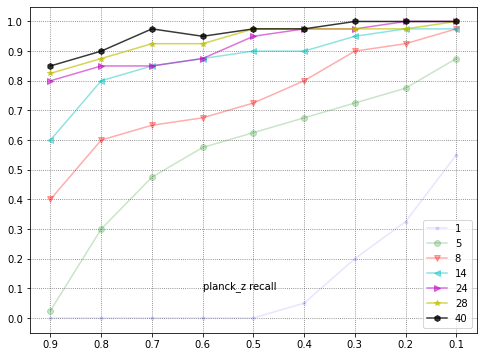
\includegraphics[width=\linewidth]{p} & 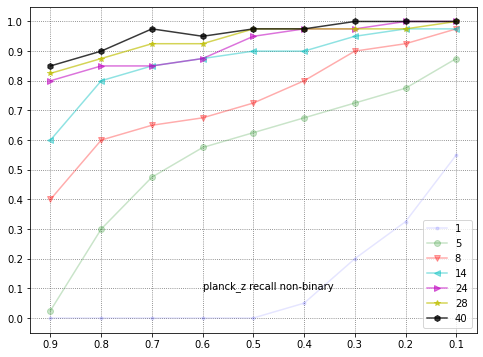
\includegraphics[width=\linewidth]{p_non_binary}\\ 
            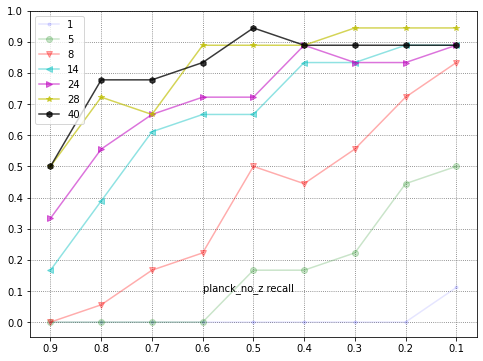
\includegraphics[width=\linewidth]{pnz} & 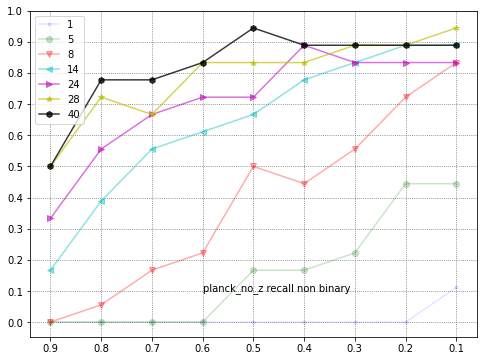
\includegraphics[width=\linewidth]{pnz_non_binary}\\ 
            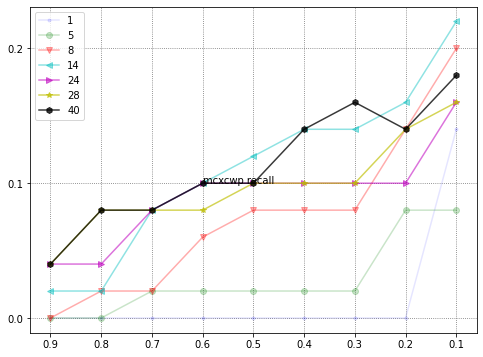
\includegraphics[width=\linewidth]{m} & 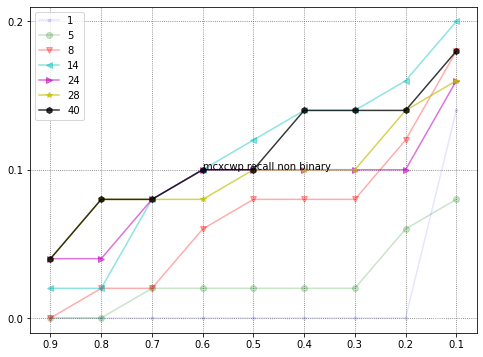
\includegraphics[width=\linewidth]{m_non_binary}\\ 
            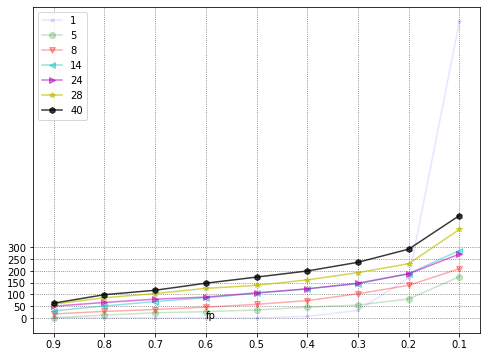
\includegraphics[width=\linewidth]{fp} & 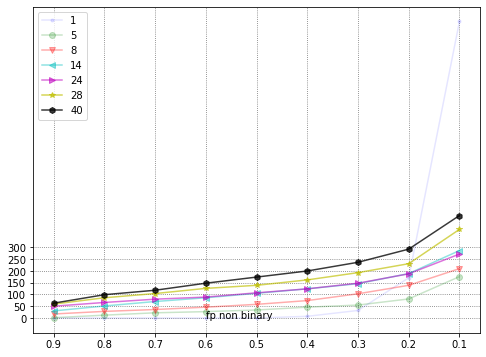
\includegraphics[width=\linewidth]{fp_non_binary}\\ 
        \end{tabular}
    \end{table}
    \newpage
    \begin{table}[h!]
        \begin{tabular}{p{0.45\linewidth}p{0.45\linewidth}}
            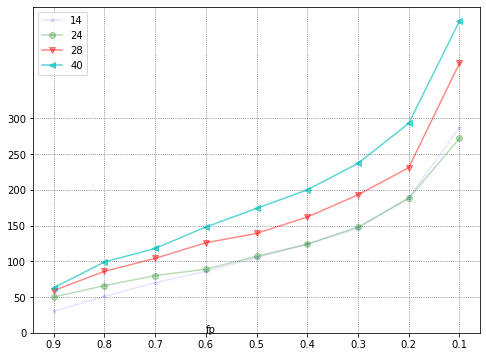
\includegraphics[width=\linewidth]{fp1} & 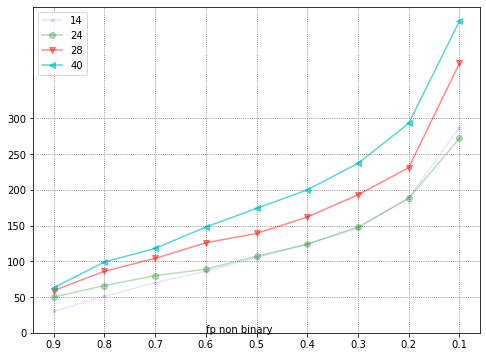
\includegraphics[width=\linewidth]{fp1_non_binary}\\ 
        \end{tabular}
    \end{table}
\end{document}
